\documentclass{IEEEtran}
\usepackage[utf8]{inputenc}
%\usepackage{fullpage}

\usepackage{amsmath}
\usepackage{graphicx}
\usepackage[colorinlistoftodos]{todonotes}
\usepackage[colorlinks=true, allcolors=blue]{hyperref}
\usepackage{mathtools}
\usepackage{latexsym}

\title{MeasureMesh: An Open Source Hardware/Software Platform for Flexible Data Logging}
\author{Matt Ruffner}
\date{}
\begin{document}

\maketitle

%%%%%%%%% ABSTRACT
% \begin{abstract}
% hello
% \end{abstract}



%%%%%%%%%%%%%%%%%%%%%%%%%%%%%
%%%%%%%%%%%%%%%%%%%%%%%%%%%%%
%%%%%%%%%%%%%%%%%%%%%%%%%%%%%
%%%%%%%%%%%%%%%%%%%%%%%%%%%%%
\section{Introduction}
 The Lora Alliance is a not profit association promoting the adoption of a Low Power Wide Area Network (LPWAN) IoT standard knows as Long Range WAN (LoRaWAN). It is a viable platform for low bandwidth, low power remote sensing applications. Over 100 complying companies adopt hardware standards including adaptive bitrate and encryption schemes specific to the LoRaWAN protocol.
 
LoRaWAN is commonly utilized for remote sensing applications including environmental and livestock monitoring~\cite{WuFan2018WAwI,IkhsanMukhammadGufron2018MLGf}. The LoRa standard is designed to be a low power solution, with longer range than traditional wireless means of communication (WiFi, Bluetooth, Zigbee, Z-Wave, etc.). It follows that compared to other wireless protocols, LoRa has significantly lower bandwidth and throughput~\cite{WuFan2018WAwI}. Performance measurements of certain LoRa chipsets have concluded that longer ranges are acheivable in a rural setting with the lowest data rates, and that range in urban settings is less, requiring lower data rates at shorter distances than in rural settings~\cite{RamonSanchez-Iborra2018PEoL}. This suggests that dynamic tuning of the radio parameters is necessary based on deployment location. 

MeasureMesh builds on this LPWAN technology to providing a simple, adaptable hardware and software platform that facilitates easy adoption for custom remote sensing networks. By using off the shelf radios and control units for node and gateway hardware, quick time-to-implementation is acheived, allowing for more focus and customization on sensing needs. The gateway utilizes internet protocol for communicating with a server back-end. For the purposes of this paper, a simple sensor data storage back-end and plotting front-end will be implemented.
%%%%%%%%%%%%%%%%%%%%%%%%%%%%%
%%%%%%%%%%%%%%%%%%%%%%%%%%%%%
%%%%%%%%%%%%%%%%%%%%%%%%%%%%%
%%%%%%%%%%%%%%%%%%%%%%%%%%%%%
\section{Project Overview} 

MeasureMesh consists of a varying number of nodes which communicate to a gateway via LoRa packet radios. The gateway then logs collected data to a cloud databse via internet. Figure \ref{fig:mmoverview} shows the MeasureMesh Implementation of a typical LoRa network topology\footnote{https://lora-alliance.org/about-lorawan}, along with chosen implementation hardware.



\begin{figure}[h!]
    \centering
    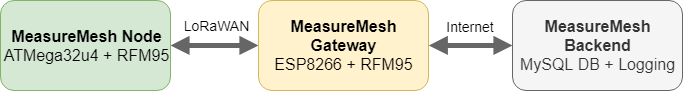
\includegraphics[width=8cm]{images/ComonentOverview.png}
    \caption{Caption}
    \label{fig:mmoverview}
\end{figure}


There are five major components of MeasureMesh, they can be seen listed in Table \ref{tab:schedule}, along with their completion status. MeasureMesh nodes consist of an Adafruit Radiofruit ATMega32u4 (Arduino programmable), with an on-board RFM95 LoRa compliant radio module \footnote{https://www.adafruit.com/product/3078}. This Radiofruit also includes a LiPo battery charger and USB connection for programming. In order to house these components, a 3D-printable enclosure was designed in CAD. This enclosure can be seen in Fig. \ref{fig:enclosure}. The 3D printed version of this enclosure, with the Node hardware inside, can be seen in Fig. \ref{fig:nodeproto}. 

\begin{figure}
    \centering
    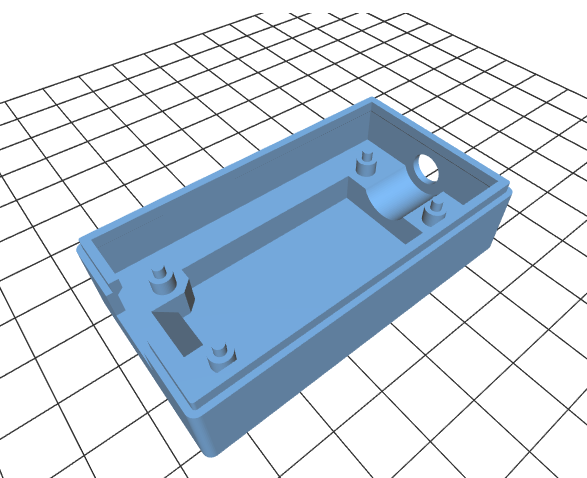
\includegraphics[width=8cm]{images/NodeEnclosure}
    \caption{Rendering of CAD model for MeasureMesh Node enclosure. Not shown: the accompanying lid that was designed.}
    \label{fig:enclosure}
\end{figure}

\begin{figure}
    \centering
    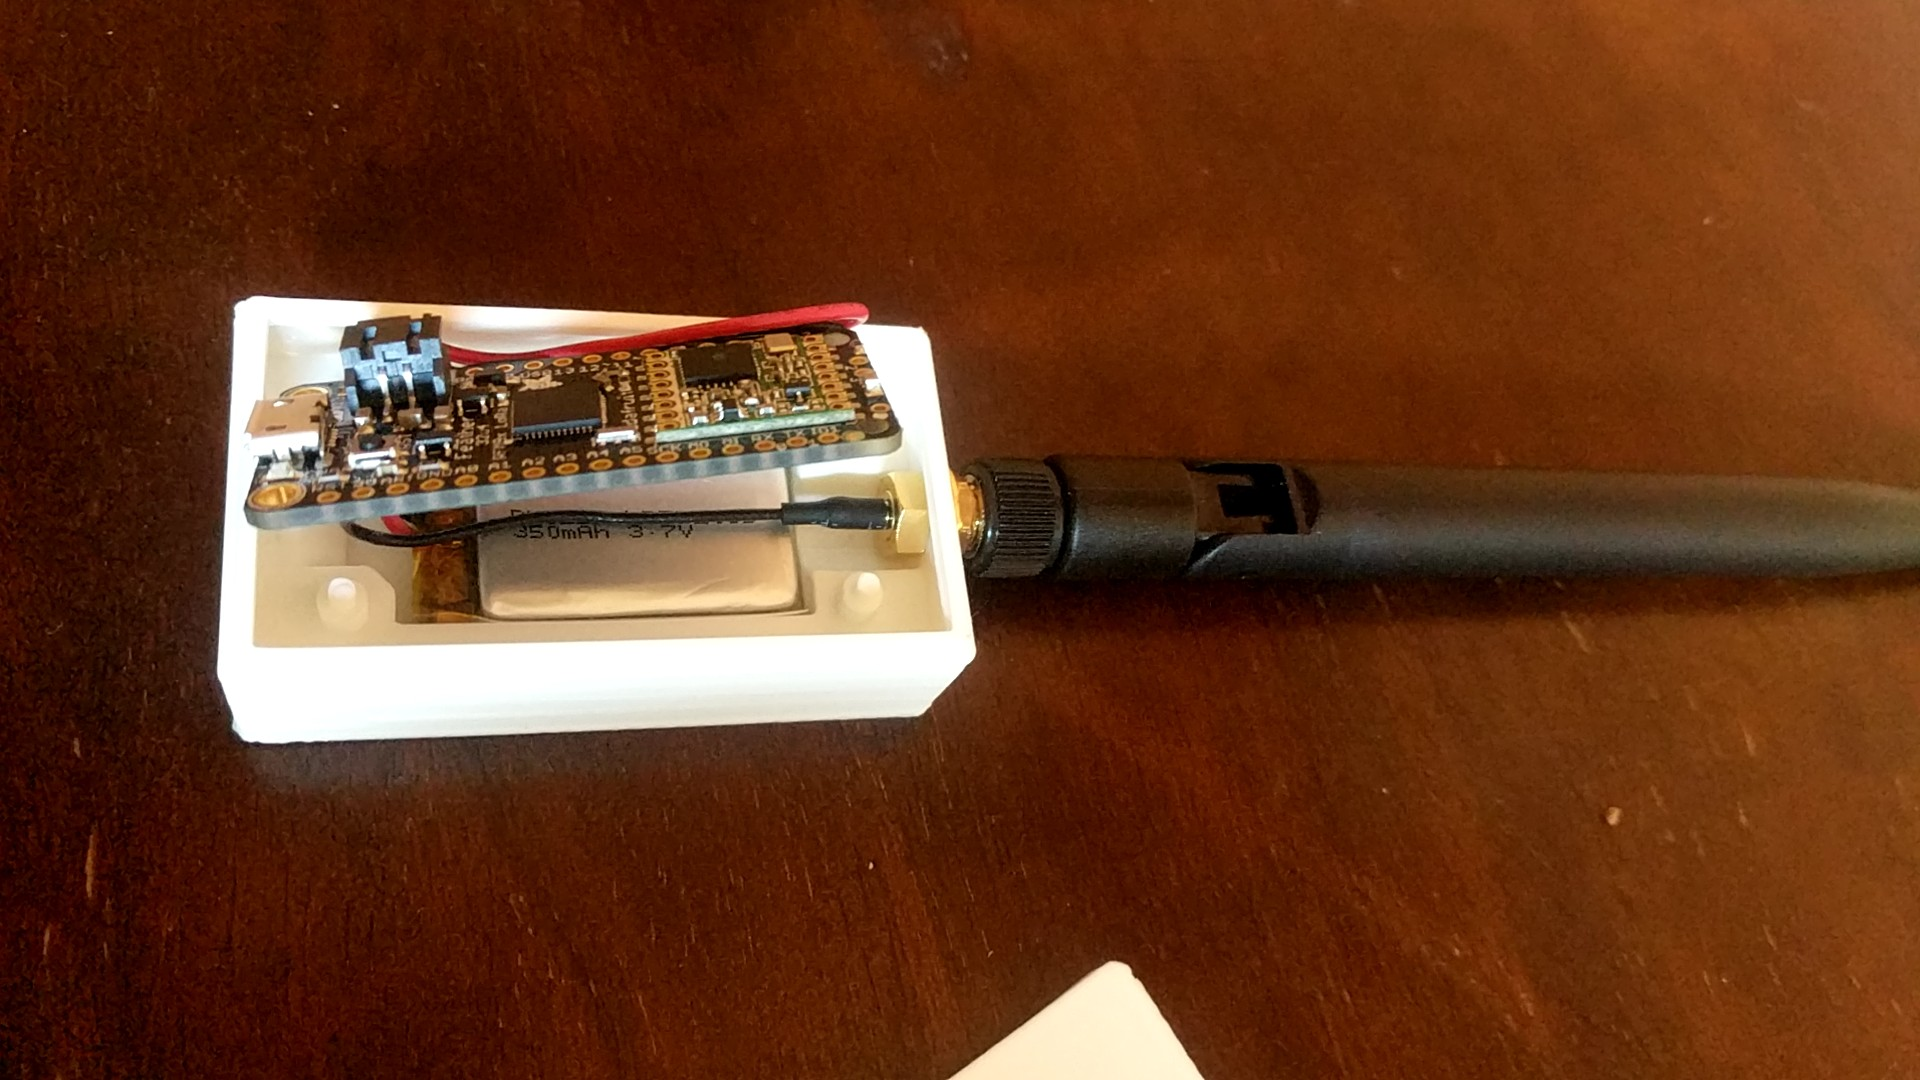
\includegraphics[width=8cm]{images/nodePrototype}
    \caption{MeasureMesh Node prototype, with enclosure, battery and antenna.}
    \label{fig:nodeproto}
\end{figure}

Describe the overall functionality along with the constituent modules of your project, as envisioned in the final product. Clearly describe different hardware and software parts/modules used or to be used. Use block diagrams, concept diagrams, graphs, flow-charts, algorithms, demo pictures, etc., to aid your description when appropriate.

%%%%%%%%%%%%%%%%%%%%%%%%%%%%%
%%%%%%%%%%%%%%%%%%%%%%%%%%%%%
%%%%%%%%%%%%%%%%%%%%%%%%%%%%%
%%%%%%%%%%%%%%%%%%%%%%%%%%%%%
\section{Projected Task Schedule} 
Divide your project into deliverable tasks and briefly describe the goals and outcomes of each task. For each task, describe an estimated time-line and workload division (in case of group projects). Clearly distinguish completed tasks from to-do tasks.

There are several deliverables with this project, the first of which are the hardware components of the nodes and gateway. As of now, there exists functional hardware for a single node as well as a single gateway. By the end of the semester I plan to have more than one node device for a more distributed system.

This leaves firmware and software milestones for the remainder of the semester. Table \ref{tab:schedule} shows a tentative schedule for the completion of remain project chunks, as well as the status of task items already finished. The back-end software depends on the completion and operation of the gateway and node firmwares, so it is scheduled to be completed last.

\begin{table}[h!]
    \centering
    \begin{tabular}{l|l}
    Component & Status and ECD \\
    \hline
    \hline
    Node hardware     &  Completed \\
    Gateway hardware  &  Completed \\
    Node firmware     & In progress, ECD 4/5/2019 \\
    Gateway firmware  & In progress, ECD 4/10/2019 \\
    Backend software  & In progress, ECD 4/20/2019
    \end{tabular}
    \vspace{2mm}
    \caption{Project components and their Expected Completion Date (ECD), if not already completed. }
    \label{tab:schedule}
\end{table}



%%%%%%%%%%%%%%%%%%%%%%%%%%%%%
%%%%%%%%%%%%%%%%%%%%%%%%%%%%%
%%%%%%%%%%%%%%%%%%%%%%%%%%%%%
%%%%%%%%%%%%%%%%%%%%%%%%%%%%%
\section{Learning Outcome}

What new did you learn for this project? Describe.



\bibliographystyle{ieeetr}
\bibliography{refs.bib}

\end{document}
